% CSC1181 Group 12 report. Two columns, A4, 11 pt, 2 cm margins.
% Build: cd report/template && tectonic main.tex
% Section text lives in sections/*.tex. Figures are read from report/.
\documentclass[11pt,a4paper,twocolumn]{article}

\usepackage[T1]{fontenc}
\usepackage[utf8]{inputenc}
\usepackage{lmodern}
\usepackage[a4paper,margin=2cm,columnsep=0.7cm]{geometry}
\usepackage{graphicx}
\usepackage{booktabs}
\usepackage{tabularx}
\usepackage{caption}
\usepackage[hidelinks]{hyperref}
\usepackage{xurl}

% Figures sit in report/, one level up from this file.
\graphicspath{{../}{./}}

% Compact, plain headings. Unnumbered so the heading text is exactly as agreed.
\setcounter{secnumdepth}{0}
\makeatletter
\renewcommand\section{\@startsection{section}{1}{\z@}%
  {1.6ex \@plus .4ex \@minus .2ex}{0.8ex}{\normalfont\large\bfseries}}
\makeatother
\setlength{\parskip}{0pt}
\captionsetup{labelfont=bf,skip=4pt}
\setlength{\textfloatsep}{10pt plus 2pt minus 2pt}
\setlength{\dbltextfloatsep}{10pt plus 2pt minus 2pt}
\renewcommand{\dbltopfraction}{0.85}
\renewcommand{\dblfloatpagefraction}{0.8}
\setcounter{dbltopnumber}{2}

% Where the section text comes from. dummy_test.tex sets this to "dummy".
\providecommand{\slotdir}{sections}
\raggedbottom
\renewcommand\refname{Bibliography}

\newcommand{\codelink}{https://github.com/neuralnomad26/causal-uplift}

\begin{document}

\twocolumn[{%
  \begin{center}
    {\LARGE\bfseries Who Actually Benefits? Causal Machine Learning for Targeted Intervention\par}
    \vspace{0.6em}
    {\large CSC1181, Group 12\par}
    \vspace{0.3em}
    Code: \url{\codelink}\par
  \end{center}
  \vspace{0.4em}
  \input{\slotdir/roles}
  \vspace{0.2em}
  \section{Abstract}
  \input{\slotdir/abstract}
  \vspace{0.4em}
}]

% Figures span both columns. A two column figure can only appear at the top of a page
% AFTER the one where it is defined, so they are defined early, right after the Abstract.
% Refer to them in the text as Figure~\ref{fig:qini} and so on.
\begin{figure*}[tp]
  \centering
  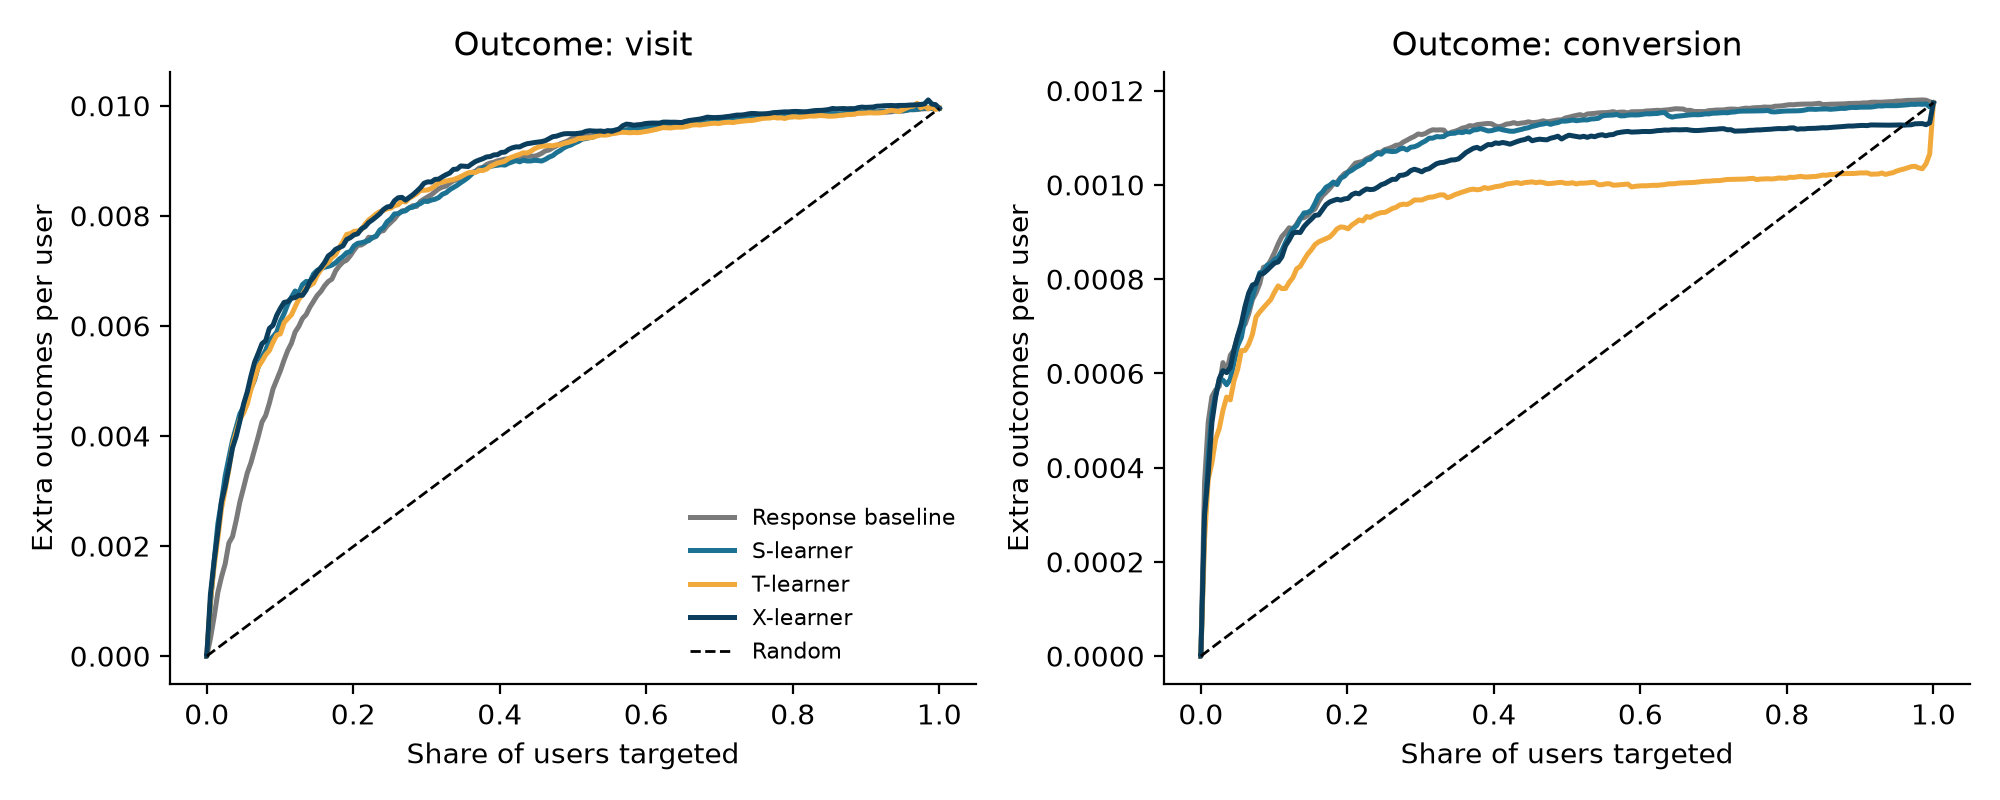
\includegraphics[width=\textwidth]{qini_curves.png}
  \caption{Qini curves on the 2M row holdout, for visits (left) and conversions (right).
  The x axis is the share of users targeted, ranked by each model's score. The y axis is the
  extra outcomes per user over targeting nobody. The dashed line is random targeting; a higher
  curve is a better ranking.}
  \label{fig:qini}
\end{figure*}

\begin{figure*}[tp]
  \centering
  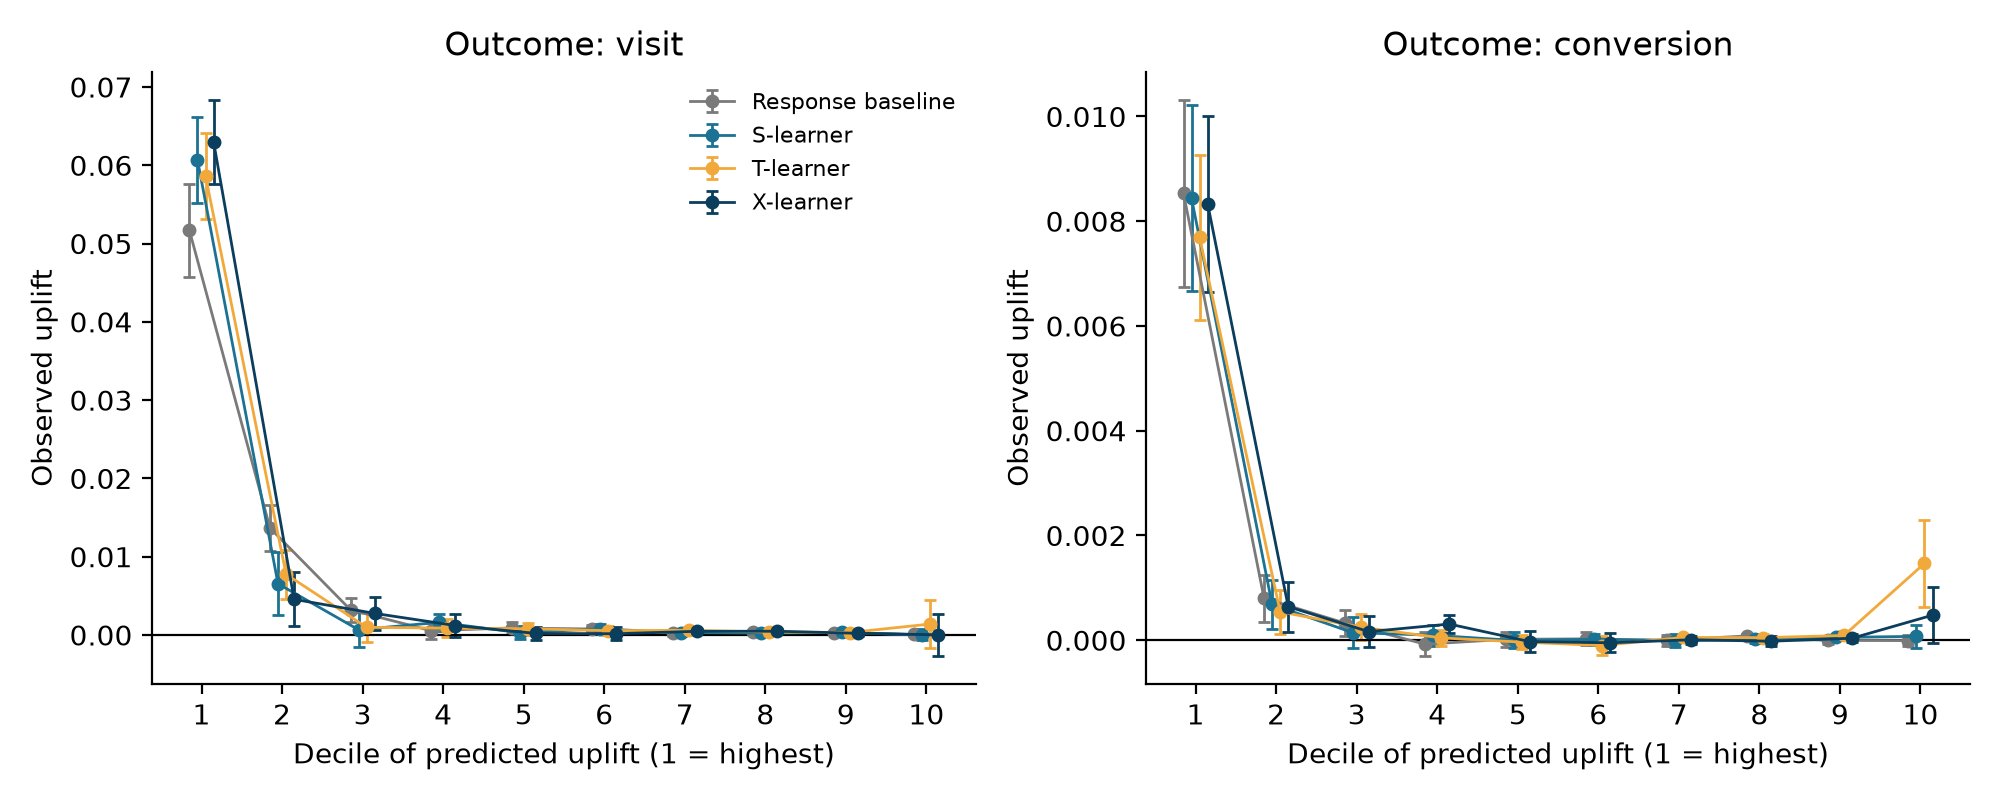
\includegraphics[width=\textwidth]{uplift_by_decile.png}
  \caption{Observed uplift by decile of predicted uplift (1 = highest), for visits (left) and
  conversions (right). Each point is the treated minus control outcome rate in that group, with
  a 95\% interval ($\pm 1.96$ standard errors). A good model is high in decile 1 and falls after.}
  \label{fig:decile}
\end{figure*}

\begin{figure*}[tp]
  \centering
  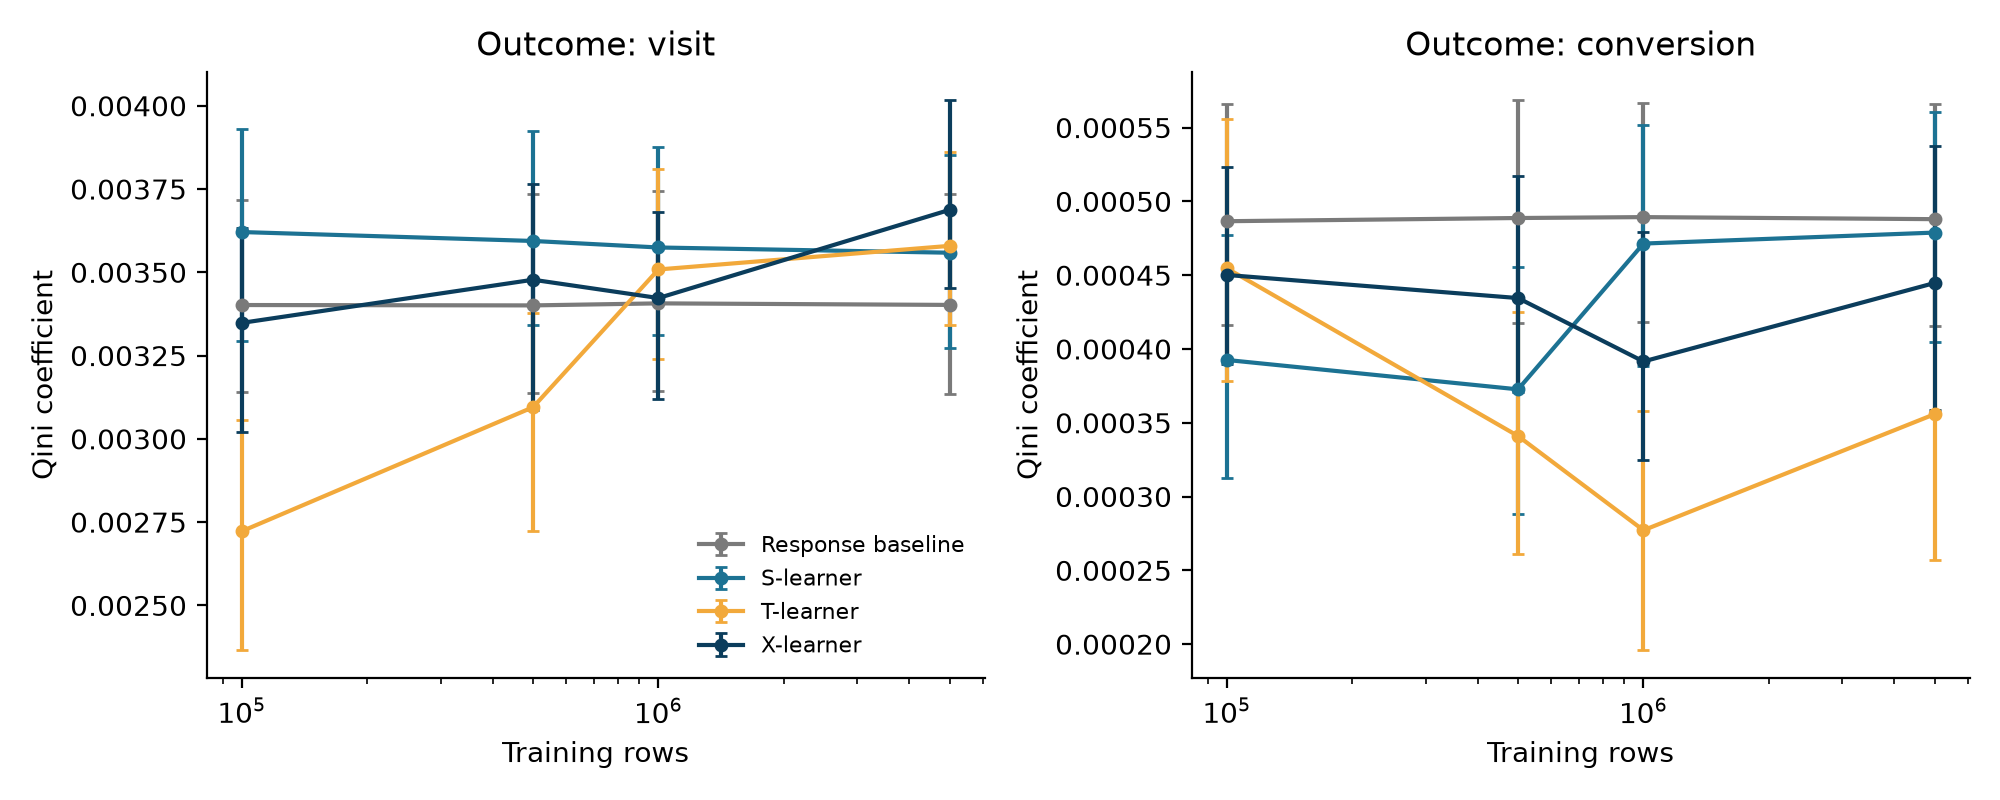
\includegraphics[width=\textwidth]{size_curve.png}
  \caption{Qini coefficient against the number of training rows (log scale), for visits (left)
  and conversions (right). Error bars are 95\% bootstrap intervals. The grey line is the response baseline.}
  \label{fig:size}
\end{figure*}

\begin{figure*}[tp]
  \centering
  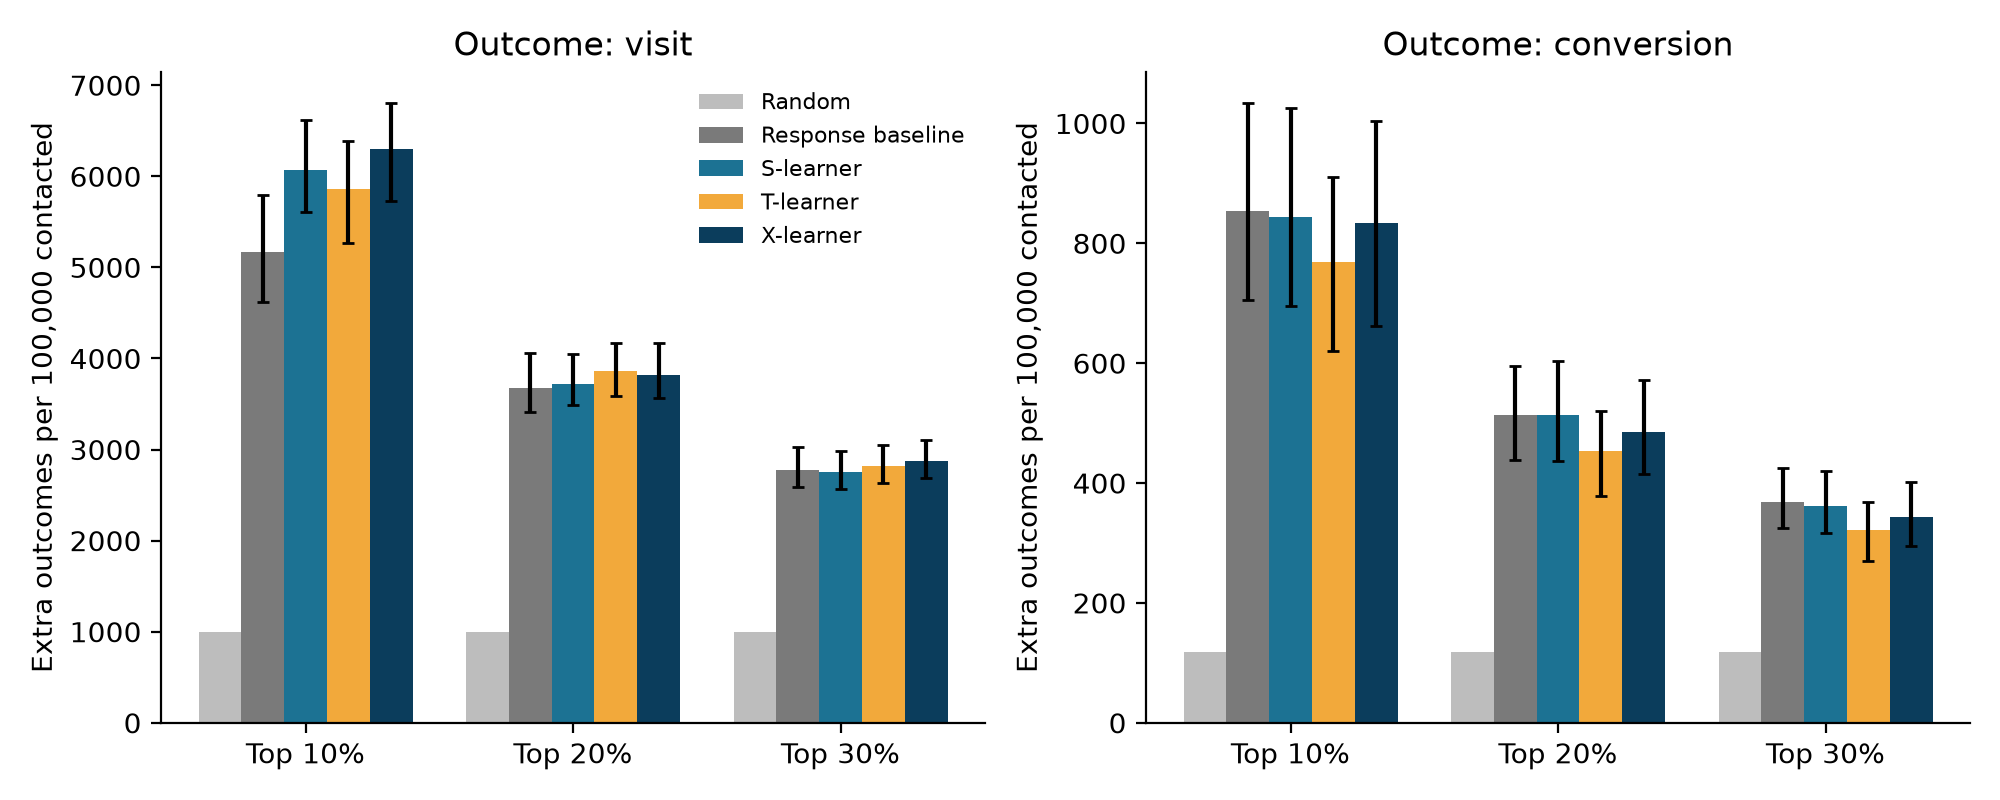
\includegraphics[width=\textwidth]{policy_simulation.png}
  \caption{Policy simulation: extra outcomes per 100,000 users contacted when each policy targets
  the top 10, 20 or 30\% of users, for visits (left) and conversions (right). Error bars are 95\%
  bootstrap intervals; random targeting has none.}
  \label{fig:policy}
\end{figure*}

\section{Problem and data}
\input{\slotdir/problem_and_data}

\section{Literature review}
\input{\slotdir/literature_review}

\section{Methods}
\input{\slotdir/methods}

\section{Results}
\input{\slotdir/results}

\section{Analysis and discussion}
\input{\slotdir/analysis_and_discussion}

\section{Ethical and legal considerations}
\input{\slotdir/ethics_and_legal}

\section{Conclusion and future work}
\input{\slotdir/conclusion}

% thebibliography prints its own heading (renamed to Bibliography above).
\input{\slotdir/references}

\end{document}
